%%
%% This is file `sample-acmlarge.tex',
%% generated with the docstrip utility.
%%
%% The original source files were:
%%
%% samples.dtx  (with options: `acmlarge')
%% 
%% IMPORTANT NOTICE:
%% 
%% For the copyright see the source file.
%% 
%% Any modified versions of this file must be renamed
%% with new filenames distinct from sample-acmlarge.tex.
%% 
%% For distribution of the original source see the terms
%% for copying and modification in the file samples.dtx.
%% 
%% This generated file may be distributed as long as the
%% original source files, as listed above, are part of the
%% same distribution. (The sources need not necessarily be
%% in the same archive or directory.)
%%
%%
%% Commands for TeXCount
%TC:macro \cite [option:text,text]
%TC:macro \citep [option:text,text]
%TC:macro \citet [option:text,text]
%TC:envir table 0 1
%TC:envir table* 0 1
%TC:envir tabular [ignore] word
%TC:envir displaymath 0 word
%TC:envir math 0 word
%TC:envir comment 0 0
%%
%%
%% The first command in your LaTeX source must be the \documentclass
%% command.
%%
%% For submission and review of your manuscript please change the
%% command to \documentclass[manuscript, screen, review]{acmart}.
%%
%% When submitting camera ready or to TAPS, please change the command
%% to \documentclass[sigconf]{acmart} or whichever template is required
%% for your publication.
%%
%%
\documentclass[acmlarge]{acmart}
\usepackage{lipsum}
%\usepackage{amsmath}
%\usepackage{amssymb}
%\usepackage{graphicx}
\usepackage[linesnumbered]{algorithm2e}

%%
%% \BibTeX command to typeset BibTeX logo in the docs
\AtBeginDocument{%
  \providecommand\BibTeX{{%
    Bib\TeX}}}

%% Rights management information.  This information is sent to you
%% when you complete the rights form.  These commands have SAMPLE
%% values in them; it is your responsibility as an author to replace
%% the commands and values with those provided to you when you
%% complete the rights form.
\setcopyright{acmcopyright}
\copyrightyear{2022}
\acmYear{2022}
\acmDOI{XXXXXXX.XXXXXXX}


%%
%% These commands are for a JOURNAL article.
\acmJournal{POMACS}
\acmVolume{37}
\acmNumber{4}
\acmArticle{111}
\acmMonth{8}

%%
%% Submission ID.
%% Use this when submitting an article to a sponsored event. You'll
%% receive a unique submission ID from the organizers
%% of the event, and this ID should be used as the parameter to this command.
%%\acmSubmissionID{123-A56-BU3}

%%
%% For managing citations, it is recommended to use bibliography
%% files in BibTeX format.
%%
%% You can then either use BibTeX with the ACM-Reference-Format style,
%% or BibLaTeX with the acmnumeric or acmauthoryear sytles, that include
%% support for advanced citation of software artefact from the
%% biblatex-software package, also separately available on CTAN.
%%
%% Look at the sample-*-biblatex.tex files for templates showcasing
%% the biblatex styles.
%%

%%
%% The majority of ACM publications use numbered citations and
%% references.  The command \citestyle{authoryear} switches to the
%% "author year" style.
%%
%% If you are preparing content for an event
%% sponsored by ACM SIGGRAPH, you must use the "author year" style of
%% citations and references.
%% Uncommenting
%% the next command will enable that style.
%%\citestyle{acmauthoryear}


%%
%% end of the preamble, start of the body of the document source.
\begin{document}

%%
%% The "title" command has an optional parameter,
%% allowing the author to define a "short title" to be used in page headers.
\title{CSE6140 Final Project}

%%
%% The "author" command and its associated commands are used to define
%% the authors and their affiliations.
%% Of note is the shared affiliation of the first two authors, and the
%% "authornote" and "authornotemark" commands
%% used to denote shared contribution to the research.
\author{Avery Bodenstein}
\authornote{All authors contributed equally to this research.}
\email{abodenstein3@gatech.edu}
\affiliation{%
  \institution{Georgia Institute of Technology}
  \streetaddress{North Ave NW}
  \city{Atlanta}
  \state{Georgia}
  \country{USA}
  \postcode{30332}
}

\author{Adrian Thinnyun}
\authornotemark[1]
\affiliation{%
	\institution{Georgia Institute of Technology}
	\streetaddress{North Ave NW}
	\city{Atlanta}
	\state{Georgia}
	\country{USA}
	\postcode{30332}
}

\author{Jai Jacob}
\authornotemark[1]
\affiliation{%
	\institution{Georgia Institute of Technology}
	\streetaddress{North Ave NW}
	\city{Atlanta}
	\state{Georgia}
	\country{USA}
	\postcode{30332}
}

\author{Zheyi Zhang}
\authornotemark[1]
\affiliation{%
	\institution{Georgia Institute of Technology}
	\streetaddress{North Ave NW}
	\city{Atlanta}
	\state{Georgia}
	\country{USA}
	\postcode{30332}
}


%%
%% The abstract is a short summary of the work to be presented in the
%% article.
\begin{abstract}
  A clear and well-documented \LaTeX\ document is presented as an
  article formatted for publication by ACM in a conference proceedings
  or journal publication. Based on the ``acmart'' document class, this
  article presents and explains many of the common variations, as well
  as many of the formatting elements an author may use in the
  preparation of the documentation of their work.
\end{abstract}

%%
%% The code below is generated by the tool at http://dl.acm.org/ccs.cfm.
%% Please copy and paste the code instead of the example below.
%%
\begin{CCSXML}
	<ccs2012>
	<concept>
	<concept_id>10003752.10003809.10003635</concept_id>
	<concept_desc>Theory of computation~Graph algorithms analysis</concept_desc>
	<concept_significance>500</concept_significance>
	</concept>
	<concept>
	<concept_id>10003752.10003809.10011254.10011256</concept_id>
	<concept_desc>Theory of computation~Branch-and-bound</concept_desc>
	<concept_significance>500</concept_significance>
	</concept>
	<concept>
	<concept_id>10003752.10003809.10003636</concept_id>
	<concept_desc>Theory of computation~Approximation algorithms analysis</concept_desc>
	<concept_significance>500</concept_significance>
	</concept>
	</ccs2012>
\end{CCSXML}

\ccsdesc[500]{Theory of computation~Graph algorithms analysis}
\ccsdesc[500]{Theory of computation~Branch-and-bound}
\ccsdesc[500]{Theory of computation~Approximation algorithms analysis}

%%
%% Keywords. The author(s) should pick words that accurately describe
%% the work being presented. Separate the keywords with commas.
\keywords{minimum vertex cover, spanning, topology, heuristics}

\received{4 December 2022}

%%
%% This command processes the author and affiliation and title
%% information and builds the first part of the formatted document.
\maketitle

\section{Introduction}

short summary of the problem, the approach and the results you have obtained

\lipsum[2-4]


\section{Problem Definition}

formal definition of the problem

\lipsum[2-4]


\section{Related Work}

a short survey of existing work on the same problem, and important results in theory
and practice

\lipsum[2-4]

\section{Algorithms}

Detailed description of each algorithm you have implemented, with pseudo-code, approx-
imation guarantee (if any), time and space complexities, etc. What are the potential strengths and
weaknesses of each type of approach? Did you use any kind of automated tuning or configuration for
your local search? Why and how you chose your local search approaches and their components? Please
cite any sources of information that you used to inform your algorithm design

\subsection{Branch and Bound}

\subsubsection{Description}

\lipsum[1]

\subsubsection{Pseudo Code}

\begin{algorithm}[H]
	\caption{merge}
	\SetAlgoLined
	\KwData{B,C}
	$n_a$ = 0\;
	i = len(B)\;
	j = len(C)\;
	A = [0]*(i+j-2)\;
	\For{l = i+j-2; l $\geq$ 0; l-=1}{
		\uIf{i == 0}{
			A[0:l] = C[0:j]\;
			return (A,$n_a$)
		}
		\uElseIf{j == 0}{
			A[0:l] = B[0:i]\;
			return (A,$n_a$)
		}
		
		\uIf{C[j-1] $\geq$ B[i-1] }{
			A[l] = C[j-1]\;
			j = j-1\;
		}
		\uElse{
			A[l] = B[i-1]\;
			$n_a$ = $n_a$ + j\;
			i = i-1\;
		}
	}
	return (A,$n_a$)
\end{algorithm}

\subsubsection{Algorithm Analysis}

\lipsum[1]

\subsection{Construction Heuristic}

\subsubsection{Description}

\lipsum[1]

\subsubsection{Pseudo Code}

\begin{algorithm}[H]
	\caption{merge}
	\SetAlgoLined
	\KwData{B,C}
	$n_a$ = 0\;
	i = len(B)\;
	j = len(C)\;
	A = [0]*(i+j-2)\;
	\For{l = i+j-2; l $\geq$ 0; l-=1}{
		\uIf{i == 0}{
			A[0:l] = C[0:j]\;
			return (A,$n_a$)
		}
		\uElseIf{j == 0}{
			A[0:l] = B[0:i]\;
			return (A,$n_a$)
		}
		
		\uIf{C[j-1] $\geq$ B[i-1] }{
			A[l] = C[j-1]\;
			j = j-1\;
		}
		\uElse{
			A[l] = B[i-1]\;
			$n_a$ = $n_a$ + j\;
			i = i-1\;
		}
	}
	return (A,$n_a$)
\end{algorithm}

\subsubsection{Algorithm Analysis}

\lipsum[1]

\subsection{Local Search 1 (specific descriptor)}

\subsubsection{Description}

\lipsum[1]

\subsubsection{Pseudo Code}

\begin{algorithm}[H]
	\caption{merge}
	\SetAlgoLined
	\KwData{B,C}
	$n_a$ = 0\;
	i = len(B)\;
	j = len(C)\;
	A = [0]*(i+j-2)\;
	\For{l = i+j-2; l $\geq$ 0; l-=1}{
		\uIf{i == 0}{
			A[0:l] = C[0:j]\;
			return (A,$n_a$)
		}
		\uElseIf{j == 0}{
			A[0:l] = B[0:i]\;
			return (A,$n_a$)
		}
		
		\uIf{C[j-1] $\geq$ B[i-1] }{
			A[l] = C[j-1]\;
			j = j-1\;
		}
		\uElse{
			A[l] = B[i-1]\;
			$n_a$ = $n_a$ + j\;
			i = i-1\;
		}
	}
	return (A,$n_a$)
\end{algorithm}

\subsubsection{Algorithm Analysis}

\lipsum[1]

\subsection{Local Search 2 (specific descriptor)}

\subsubsection{Description}

\lipsum[1]

\subsubsection{Pseudo Code}

\begin{algorithm}[H]
	\caption{merge}
	\SetAlgoLined
	\KwData{B,C}
	$n_a$ = 0\;
	i = len(B)\;
	j = len(C)\;
	A = [0]*(i+j-2)\;
	\For{l = i+j-2; l $\geq$ 0; l-=1}{
		\uIf{i == 0}{
			A[0:l] = C[0:j]\;
			return (A,$n_a$)
		}
		\uElseIf{j == 0}{
			A[0:l] = B[0:i]\;
			return (A,$n_a$)
		}
		
		\uIf{C[j-1] $\geq$ B[i-1] }{
			A[l] = C[j-1]\;
			j = j-1\;
		}
		\uElse{
			A[l] = B[i-1]\;
			$n_a$ = $n_a$ + j\;
			i = i-1\;
		}
	}
	return (A,$n_a$)
\end{algorithm}

\subsubsection{Algorithm Analysis}

\lipsum[1]

\section{Empirical Evaluation}

a detailed description of your platform (CPU, RAM, language, compiler, etc.),
experimental procedure, evaluation criteria and obtained results (plots, tables, etc.). What is the
lower bound on the optimal solution quality that you can drive from the results of your approximation
algorithm and how far is it from the true optimum? How about from your branch-and-bound?

\section{Discussion}

a comparative analysis of how different algorithms perform with respect to your evaluation
criteria, or expected time complexity, etc


\section{Conclusion}



\section{Math Equations}
You may want to display math equations in three distinct styles:
inline, numbered or non-numbered display.  Each of the three are
discussed in the next sections.

\subsection{Inline (In-text) Equations}
A formula that appears in the running text is called an inline or
in-text formula.  It is produced by the \textbf{math} environment,
which can be invoked with the usual
\texttt{{\char'134}begin\,\ldots{\char'134}end} construction or with
the short form \texttt{\$\,\ldots\$}. You can use any of the symbols
and structures, from $\alpha$ to $\omega$, available in
\LaTeX~\cite{Lamport:LaTeX}; this section will simply show a few
examples of in-text equations in context. Notice how this equation:
\begin{math}
  \lim_{n\rightarrow \infty}x=0
\end{math},
set here in in-line math style, looks slightly different when
set in display style.  (See next section).

\subsection{Display Equations}
A numbered display equation---one set off by vertical space from the
text and centered horizontally---is produced by the \textbf{equation}
environment. An unnumbered display equation is produced by the
\textbf{displaymath} environment.

Again, in either environment, you can use any of the symbols and
structures available in \LaTeX\@; this section will just give a couple
of examples of display equations in context.  First, consider the
equation, shown as an inline equation above:
\begin{equation}
  \lim_{n\rightarrow \infty}x=0
\end{equation}
Notice how it is formatted somewhat differently in
the \textbf{displaymath}
environment.  Now, we'll enter an unnumbered equation:
\begin{displaymath}
  \sum_{i=0}^{\infty} x + 1
\end{displaymath}
and follow it with another numbered equation:
\begin{equation}
  \sum_{i=0}^{\infty}x_i=\int_{0}^{\pi+2} f
\end{equation}
just to demonstrate \LaTeX's able handling of numbering.

\section{Figures}

The ``\verb|figure|'' environment should be used for figures. One or
more images can be placed within a figure. If your figure contains
third-party material, you must clearly identify it as such, as shown
in the example below.
\begin{figure}[h]
  \centering
  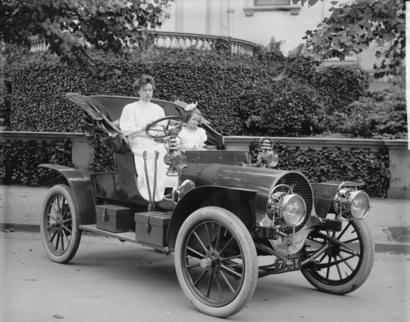
\includegraphics[width=\linewidth]{sample-franklin}
  \caption{1907 Franklin Model D roadster. Photograph by Harris \&
    Ewing, Inc. [Public domain], via Wikimedia
    Commons. (\url{https://goo.gl/VLCRBB}).}
  \Description{A woman and a girl in white dresses sit in an open car.}
\end{figure}

Your figures should contain a caption which describes the figure to
the reader.

Figure captions are placed {\itshape below} the figure.

Every figure should also have a figure description unless it is purely
decorative. These descriptions convey what’s in the image to someone
who cannot see it. They are also used by search engine crawlers for
indexing images, and when images cannot be loaded.

A figure description must be unformatted plain text less than 2000
characters long (including spaces).  {\bfseries Figure descriptions
  should not repeat the figure caption – their purpose is to capture
  important information that is not already provided in the caption or
  the main text of the paper.} For figures that convey important and
complex new information, a short text description may not be
adequate. More complex alternative descriptions can be placed in an
appendix and referenced in a short figure description. For example,
provide a data table capturing the information in a bar chart, or a
structured list representing a graph.  For additional information
regarding how best to write figure descriptions and why doing this is
so important, please see
\url{https://www.acm.org/publications/taps/describing-figures/}.

\subsection{The ``Teaser Figure''}

A ``teaser figure'' is an image, or set of images in one figure, that
are placed after all author and affiliation information, and before
the body of the article, spanning the page. If you wish to have such a
figure in your article, place the command immediately before the
\verb|\maketitle| command:
\begin{verbatim}
  \begin{teaserfigure}
    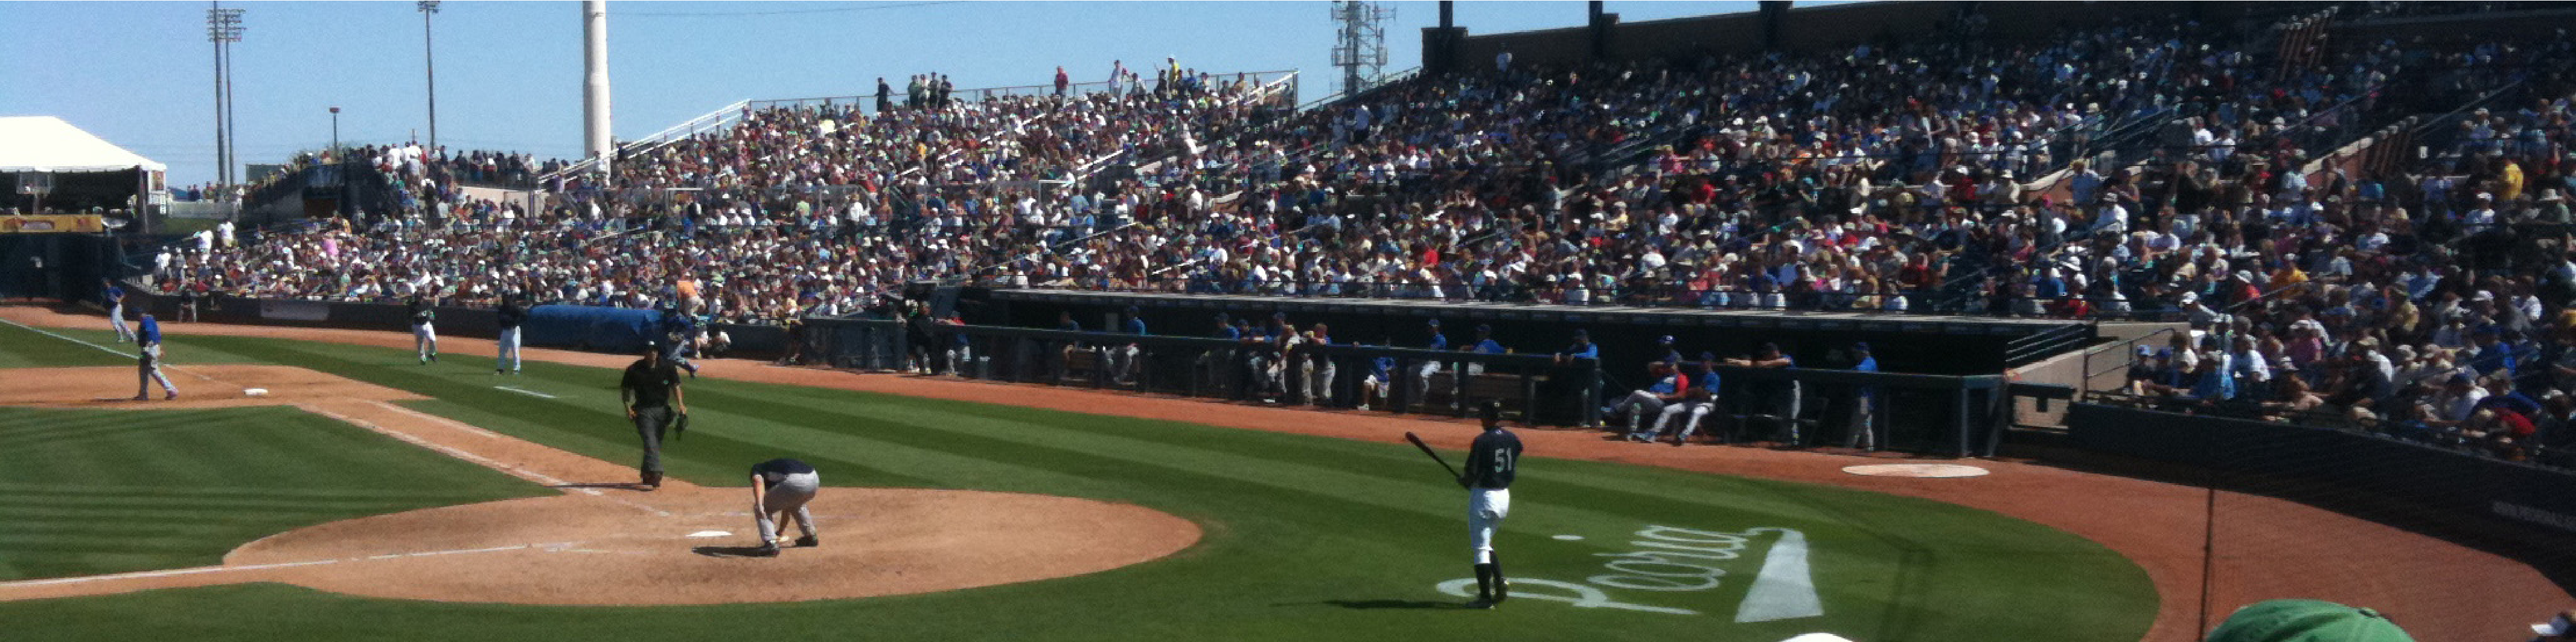
\includegraphics[width=\textwidth]{sampleteaser}
    \caption{figure caption}
    \Description{figure description}
  \end{teaserfigure}
\end{verbatim}

\section{Citations and Bibliographies}

The use of \BibTeX\ for the preparation and formatting of one's
references is strongly recommended. Authors' names should be complete
--- use full first names (``Donald E. Knuth'') not initials
(``D. E. Knuth'') --- and the salient identifying features of a
reference should be included: title, year, volume, number, pages,
article DOI, etc.

The bibliography is included in your source document with these two
commands, placed just before the \verb|\end{document}| command:
\begin{verbatim}
  \bibliographystyle{ACM-Reference-Format}
  \bibliography{bibfile}
\end{verbatim}
where ``\verb|bibfile|'' is the name, without the ``\verb|.bib|''
suffix, of the \BibTeX\ file.

Citations and references are numbered by default. A small number of
ACM publications have citations and references formatted in the
``author year'' style; for these exceptions, please include this
command in the {\bfseries preamble} (before the command
``\verb|\begin{document}|'') of your \LaTeX\ source:
\begin{verbatim}
  \citestyle{acmauthoryear}
\end{verbatim}


  Some examples.  A paginated journal article \cite{Abril07}, an
  enumerated journal article \cite{Cohen07}, a reference to an entire
  issue \cite{JCohen96}, a monograph (whole book) \cite{Kosiur01}, a
  monograph/whole book in a series (see 2a in spec. document)
  \cite{Harel79}, a divisible-book such as an anthology or compilation
  \cite{Editor00} followed by the same example, however we only output
  the series if the volume number is given \cite{Editor00a} (so
  Editor00a's series should NOT be present since it has no vol. no.),
  a chapter in a divisible book \cite{Spector90}, a chapter in a
  divisible book in a series \cite{Douglass98}, a multi-volume work as
  book \cite{Knuth97}, a couple of articles in a proceedings (of a
  conference, symposium, workshop for example) (paginated proceedings
  article) \cite{Andler79, Hagerup1993}, a proceedings article with
  all possible elements \cite{Smith10}, an example of an enumerated
  proceedings article \cite{VanGundy07}, an informally published work
  \cite{Harel78}, a couple of preprints \cite{Bornmann2019,
    AnzarootPBM14}, a doctoral dissertation \cite{Clarkson85}, a
  master's thesis: \cite{anisi03}, an online document / world wide web
  resource \cite{Thornburg01, Ablamowicz07, Poker06}, a video game
  (Case 1) \cite{Obama08} and (Case 2) \cite{Novak03} and \cite{Lee05}
  and (Case 3) a patent \cite{JoeScientist001}, work accepted for
  publication \cite{rous08}, 'YYYYb'-test for prolific author
  \cite{SaeediMEJ10} and \cite{SaeediJETC10}. Other cites might
  contain 'duplicate' DOI and URLs (some SIAM articles)
  \cite{Kirschmer:2010:AEI:1958016.1958018}. Boris / Barbara Beeton:
  multi-volume works as books \cite{MR781536} and \cite{MR781537}. A
  couple of citations with DOIs:
  \cite{2004:ITE:1009386.1010128,Kirschmer:2010:AEI:1958016.1958018}. Online
  citations: \cite{TUGInstmem, Thornburg01, CTANacmart}.
  Artifacts: \cite{R} and \cite{UMassCitations}.

\section{Acknowledgments}

Identification of funding sources and other support, and thanks to
individuals and groups that assisted in the research and the
preparation of the work should be included in an acknowledgment
section, which is placed just before the reference section in your
document.

This section has a special environment:
\begin{verbatim}
  \begin{acks}
  ...
  \end{acks}
\end{verbatim}
so that the information contained therein can be more easily collected
during the article metadata extraction phase, and to ensure
consistency in the spelling of the section heading.

Authors should not prepare this section as a numbered or unnumbered {\verb|\section|}; please use the ``{\verb|acks|}'' environment.


%%
%% The acknowledgments section is defined using the "acks" environment
%% (and NOT an unnumbered section). This ensures the proper
%% identification of the section in the article metadata, and the
%% consistent spelling of the heading.
\begin{acks}
To Robert, for the bagels and explaining CMYK and color spaces.
\end{acks}

%%
%% The next two lines define the bibliography style to be used, and
%% the bibliography file.
\bibliographystyle{ACM-Reference-Format}
\bibliography{sample-base}


\end{document}
\endinput
%%
%% End of file `sample-acmlarge.tex'.
